\subsection{Уравнение Лапласа в криволинейных ортогональных (полярных, цилиндрических, сферических) координатах.}
\label{sec:14}

%Самарский стр. 298
%aut: Денис


Выведем вырадение для оператора Лапласа в ортогональной криволинейной системе координат. Пусть в пространстве вместо декартовых координат $x, y, z$ введены криволинейные координаты $q_{1}, q_{2}, q_{3}$ с помощью соотношений
\[
q_{1}=f_{1}(x, y, z), \quad q_{2}=f_{2}(x, y, z), \quad q_{3}=f_{3}(x, y, z),
\]
разрешая которые относительно $x, y, z$, можно написать
\[
x=\varphi_{1}\left(q_{1}, q_{2}, q_{3}\right), \quad y=\varphi_{2}\left(q_{1}, q_{2}, q_{3}\right), \quad z=\varphi_{3}\left(q_{1}, q_{2}, q_{3}\right) .
\]

Полагая $q_{1}=C_{1}, q_{2}=C_{2}, q_{3}=C_{3}$, где $C_{1}, C_{2}, C_{3}$ - постоянные, получим три семейства координатных поверхностей:
\[
f_{1}(x, y, z)=C_{1}, \quad f_{2}(x, y, z)=C_{2}, \quad f_{3}(x, y, z)=C_{3} .
\]
\begin{figure}[h!]
	\centering
	\scalebox{0.5}{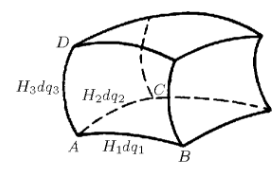
\includegraphics{img/graph}}
\end{figure}

Рассмотрим элемент объема в новых координатах, ограниченный тремя парами координатных поверхностей. Вдоль ребра $A B$ $q_{2}=$ const, $q_{3}=$ const, вдоль $A D \quad q_{1}=$ const, $q_{2}=$ const, вдоль $A C$ $q_{1}=$ const, $q_{3}=$ const. Направляющие косинусы касательной к ребрам $A B, A C$ и $A D$ пропорциональны соответственно
\[
\frac{\partial \varphi_{1}}{\partial q_{1}}, \quad \frac{\partial \varphi_{2}}{\partial q_{1}}, \quad \frac{\partial \varphi_{3}}{\partial q_{1}} ; \quad \frac{\partial \varphi_{1}}{\partial q_{2}}, \quad \frac{\partial \varphi_{2}}{\partial q_{2}}, \quad \frac{\partial \varphi_{3}}{\partial q_{2}} ; \quad \frac{\partial \varphi_{1}}{\partial q_{3}}, \quad \frac{\partial \varphi_{2}}{\partial q_{3}}, \quad \frac{\partial \varphi_{3}}{\partial q_{3}} .
\]

Условие ортогональности ребер будет иметь вид
\[
\frac{\partial \varphi_{1}}{\partial q_{i}} \frac{\partial \varphi_{1}}{\partial q_{k}}+\frac{\partial \varphi_{2}}{\partial q_{i}} \frac{\partial \varphi_{2}}{\partial q_{k}}+\frac{\partial \varphi_{3}}{\partial q_{i}} \frac{\partial \varphi_{3}}{\partial q_{k}}=0 \quad(i \neq k) .
\]

Вычислим элемент длины в новых координатах:
\[
\begin{aligned} 
	d s^{2}=d x^{2}+d y^{2}+ d z^{2}=\left(\frac{\partial \varphi_{1}}{\partial q_{1}} d q_{1}+\frac{\partial \varphi_{1}}{\partial q_{2}} d q_{2}+\frac{\partial \varphi_{1}}{\partial q_{3}} d q_{3}\right)^{2}+ \\
	+\left(\frac{\partial \varphi_{2}}{\partial q_{1}} d q_{1}+\frac{\partial \varphi_{2}}{\partial q_{2}} d q_{2}+\frac{\partial \varphi_{2}}{\partial q_{3}} d q_{3}\right)^{2}+ \\
	+\left(\frac{\partial \varphi_{3}}{\partial q_{1}} d q_{1}+\frac{\partial \varphi_{3}}{\partial q_{2}} d q_{2}+\frac{\partial \varphi_{3}}{\partial q_{3}} d q_{3}\right)^{2} .
\end{aligned}
\]

Раскрывая скобки и учитывая условия ортогональности, получаем
\[
d s^{2}=H_{1}^{2} d q_{1}^{2}+H_{2}^{2} d q_{2}^{2}+H_{3}^{2} d q_{3}^{2},
\]

где
\[
\left.\begin{aligned}
	H_{1}^{2}=\left(\frac{\partial \varphi_{1}}{\partial q_{1}}\right)^{2}+\left(\frac{\partial \varphi_{2}}{\partial q_{1}}\right)^{2}+\left(\frac{\partial \varphi_{3}}{\partial q_{1}}\right)^{2}, \\
	H_{2}^{2}=\left(\frac{\partial \varphi_{1}}{\partial q_{2}}\right)^{2}+\left(\frac{\partial \varphi_{2}}{\partial q_{2}}\right)^{2}+\left(\frac{\partial \varphi_{3}}{\partial q_{2}}\right)^{2}, \\
	H_{3}^{2}=\left(\frac{\partial \varphi_{1}}{\partial q_{3}}\right)^{2}+\left(\frac{\partial \varphi_{2}}{\partial q_{3}}\right)^{2}+\left(\frac{\partial \varphi_{3}}{\partial q_{3}}\right)^{2} \cdot
\end{aligned}\right\}
\]

Вдоль каждого из ребер элементарного объема меняется только одна координата, поэтому для длины этих ребер согласно формуле над системой будем иметь
\[
d s_{1}=H_{1} d q_{1}, \quad d s_{2}=H_{2} d q_{2}, \quad d s_{3}=H_{3} d q_{3},
\]

так что элемент объема равен
\[
d v=d s_{1} d s_{2} d s_{3}=H_{1} H_{2} H_{3} d q_{1} d q_{2} d q_{3} .
\]

Рассмотрим теперь некоторое векторное поле $\mathbf{A}(x, y, z)$. Вычислим $\operatorname{div} \mathbf{A}$, определяемую известной формулой векторного анализа
\[
\operatorname{div} \mathbf{A}=\lim _{v_{M} \rightarrow 0} \frac{\iint_{S} A_{n} d S}{v_{M}},
\]

где $S$ - поверхность, ограничивающая некоторый объем $v_{M}$, содержащий рассматриваемую точку $M$. Применим эту формулу к элементу объема $d v$, изображенному на рисунке.

Пользуясь теоремой о среднем, можно представить разность потоков вектора $\mathbf{A}$ через противоположные грани, например через правую и левую, в виде
\[
Q_{1}=\left.A_{1} d s_{2} d s_{3}\right|_{q_{1}+d q_{1}}-\left.A_{1} d s_{2} d s_{3}\right|_{q_{1}} .
\]

Принимая во внимание формулы для $ds_1, ds_2$ и $ds_3$, получим
\[
\begin{aligned}
	Q_{1}=\left[\left.H_{2} H_{3} A_{1}\right|_{q_{1}+d q_{1}}-\left.H_{2} H_{3} A_{1}\right|_{q_{1}}\right] d q_{2} d q_{3}= \\
	=\frac{\partial}{\partial q_{1}}\left(H_{2} H_{3} A_{1}\right) d q_{1} d q_{2} d q_{3} .
\end{aligned}
\]

Аналогично вычисляются две другие разности потоков через противоположные грани:
\[
\begin{aligned}
	Q_{2} & =\frac{\partial}{\partial q_{2}}\left(H_{3} H_{1} A_{2}\right) d q_{1} d q_{2} d q_{3}, \\
	Q_{3} & =\frac{\partial}{\partial q_{3}}\left(H_{1} H_{2} A_{3}\right) d q_{1} d q_{2} d q_{3} .
\end{aligned}
\]

Подставляя в формулу $\operatorname{div} \mathbf{A}$ значение $\iint_{S} A_{n} d S=Q_{1}+Q_{2}+Q_{3}$ и пользуясь формулой $dv$, получаем выражение дивергенции в криволинейных ортогональных координатах:
\[
\operatorname{div} \mathbf{A}=\frac{1}{H_{1} H_{2} H_{3}}\left[\frac{\partial}{\partial q_{1}}\left(H_{2} H_{3} A_{1}\right)+\frac{\partial}{\partial q_{2}}\left(H_{3} H_{1} A_{2}\right)+\frac{\partial}{\partial q_{3}}\left(H_{1} H_{2} A_{3}\right)\right] .
\]

Предположим, что поле А потенциальное, т. е.
\[
\mathbf{A}=\operatorname{grad} u .
\]

Тогда
\[
A_{1}=\frac{\partial u}{\partial s_{1}}=\frac{1}{H_{1}} \frac{\partial u}{\partial q_{1}} ; \quad A_{2}=\frac{1}{H_{2}} \frac{\partial u}{\partial q_{2}} ; \quad A_{3}=\frac{1}{H_{3}} \frac{\partial u}{\partial q_{3}} .
\]

Подставив в полученную чуть выше формулу для $\operatorname{div} \mathbf{A}$ выражения для $A_{1}, A_{2}, A_{3}$, получим выражение для оператора Лапласа:
\[
\begin{aligned}
	\Delta u=\operatorname{div} \operatorname{grad} u= & \frac{1}{H_{1} H_{2} H_{3}}\left[\frac{\partial}{\partial q_{1}}\left(\frac{H_{2} H_{3}}{H_{1}} \frac{\partial u}{\partial q_{1}}\right)+\right. \\
	& \left.+\frac{\partial}{\partial q_{2}}\left(\frac{H_{3} H_{1}}{H_{2}} \frac{\partial u}{\partial q_{2}}\right)+\frac{\partial}{\partial q_{3}}\left(\frac{H_{1} H_{2}}{H_{3}} \frac{\partial u}{\partial q_{3}}\right)\right] .
\end{aligned}
\]

Таким образом, уравнение Лапласа $\Delta u=0$ в ортогональных криволинейных координатах $q_{1}, q_{2}$ и $q_{3}$ записывается следующим образом:
\[
\begin{aligned}
	\frac{1}{H_{1} H_{2} H_{3}}\left[\frac{\partial}{\partial q_{1}}\right. & \left(\frac{H_{2} H_{3}}{H_{1}} \frac{\partial u}{\partial q_{1}}\right)+ \\
	& \left.+\frac{\partial}{\partial q_{2}}\left(\frac{H_{3} H_{1}}{H_{2}} \frac{\partial u}{\partial q_{2}}\right)+\frac{\partial}{\partial q_{3}}\left(\frac{H_{1} H_{2}}{H_{3}} \frac{\partial u}{\partial q_{3}}\right)\right]=0 .
\end{aligned}
\]

Рассмотрим два частных случая.

\textbf{Сферические координаты.} В этом случае $q_{1}=r, q_{2}=\theta$, $q_{3}=\varphi$ и формулы преобразования принимают вид
\[
x=r \sin \theta \cos \varphi, \quad y=r \sin \theta \sin \varphi, \quad z=r \cos \theta .
\]

Вычислим $d s^{2}$ :
\[
\begin{aligned}
	d s^{2}=(\sin \theta \cos \varphi d r+r \cos \theta \cos \varphi d \theta-r \sin \theta \sin \varphi d \varphi)^{2}+ \\
	\quad+(\sin \theta \sin \varphi d r+r \cos \theta \sin \varphi d \theta+r \sin \theta \cos \varphi d \varphi)^{2}+ \\
	\quad+(\cos \theta d r-r \sin \theta d \theta)^{2} ;
\end{aligned}
\]
после раскрытия скобок и упрощений находим
\[
d s^{2}=d r^{2}+r^{2} d \theta^{2}+r^{2} \sin ^{2} \theta d \varphi^{2},
\]
т. e.
\[
H_{1}=1, \quad H_{2}=r, \quad H_{3}=r \sin \theta .
\]

Подставив значения $H_{1}, H_{2}, H_{3}$ в формулу уравнения Лапласа, получим уравнение Лапласа в сферических координатах:
\[
\frac{1}{r^{2} \sin \theta}\left[\frac{\partial}{\partial r}\left(r^{2} \sin \theta \frac{\partial u}{\partial r}\right)+\frac{\partial}{\partial \theta}\left(\sin \theta \frac{\partial u}{\partial \theta}\right)+\frac{\partial}{\partial \varphi}\left(\frac{1}{\sin \theta} \frac{\partial u}{\partial \varphi}\right)\right]=0,
\]

или окончательно
\[
\Delta_{r, \theta, \varphi} u=\frac{1}{r^{2}} \frac{\partial}{\partial r}\left(r^{2} \frac{\partial u}{\partial r}\right)+\frac{1}{r^{2} \sin \theta} \frac{\partial}{\partial \theta}\left(\sin \theta \frac{\partial u}{\partial \theta}\right)+\frac{1}{r^{2} \sin ^{2} \theta} \frac{\partial^{2} u}{\partial \varphi^{2}}=0 .
\]

\textbf{Цилиндрические координаты.} В этом случае $q_{1}=\rho$, $q_{2}=\varphi, q_{3}=z$ и
\[
x=\rho \cos \varphi, \quad y=\rho \sin \varphi, \quad z=z,
\]

так что
\[
H_{1}=1, \quad H_{2}=\rho, \quad H_{3}=1 .
\]

Уравнение Лапласа в цилиндрических координатах принимает вид
\[
\Delta_{\rho, \varphi, z} u=\frac{1}{\rho} \frac{\partial}{\partial \rho}\left(\rho \frac{\partial u}{\partial \rho}\right)+\frac{1}{\rho^{2}} \frac{\partial^{2} u}{\partial \varphi^{2}}+\frac{\partial^{2} u}{\partial z^{2}}=0 .
\]

Если искомая функция $u$ не зависит от $z$, то уравнение упрощается:
\[
\Delta_{\rho, \varphi} u=\frac{1}{\rho} \frac{\partial}{\partial \rho}\left(\rho \frac{\partial u}{\partial \rho}\right)+\frac{1}{\rho^{2}} \frac{\partial^{2} u}{\partial \varphi^{2}}=0
\]